\labeledsection{Machine-Oriented Calculi for Propositional Logic}{sec:atp_pl0}
\commandnote{From \Thmref{thm:unsat}, we observe that \linkterm{entailment}{entailment_pl0} can be tested via \linkterm{satisfiablity}{satisfiable_ls}}

\definition{Theorem Proving}{
Given a \linkterm{formal system}{formal_system} $\tuple{\mathcal{S}, \mathcal{C}}$, where $\mathcal{C}$ is a \linkterm{calculus}{calculus_logic} and $\mathcal{S} := \langle \mathcal{L}, \mathcal{M}, \vDash \rangle$ is a \linkterm{logical system}{logical_system}, the task of \textbf{theorem proving} is the task of determining whether $\mathcal{H} \vdash_{\mathcal{C}} C$ for a \textbf{conjecture} $C \in \mathcal{L}$ and hypotheses $\mathcal{H} \subseteq \mathcal{L}$
}{theorem_proving}

\definition{Automated Theorem Proving}{
\textbf{ATP} is the automation of \linkterm{theorem proving}{theorem_proving}.
}{def:atp}

\definition{Test Calculus}{
For a given \linkterm{conjecture}{theorem_proving} $A$ and \linkterm{hypotheses}{theorem_proving} $\mathcal{H}$, a \textbf{test calculus} $\mathcal{T}$ tries to derive a \linkterm{refutation}{c_refutation} $\mathcal{H}, \neg A \vdash_{\mathcal{T}} \bot$ instead of $\mathcal{H} \vdash A$, where $\neg A$ is \linkterm{unsatisfiable}{unsatisfiable_ls} iff $A$ is \linkterm{valid}{valid_ls} and $\bot$ an \linkterm{unsatisfiable}{unsatisfiable_ls} \linkterm{proposition}{proposition}.
}{test_calculus}


\definition{Atomic Formulae}{
A \linkterm{formula}{formulae} is called \textbf{atmoic} (or an \textbf{atom}) if it does not contain logical constants, otherwise, \textbf{complex}
}{atomic_formula}

\definition{Labeled Formula}{
Let $\mathcal{S} := \langle \mathcal{L}, \mathcal{M}, \vDash \rangle$ be a \linkterm{logical system}{logical_system}, $A \in \mathcal{L}$ a formula, $L$ a \textbf{label set}, and $\alpha \in L$ a \textbf{label}, then we call a \linkterm{pair}{cartesian_product} $\tuple{A, \alpha}$ a \textbf{labeled formula} and write it as $A^{\alpha}$. For a \linkterm{set}{def:set} $\Phi$ of \linkterm{propositions}{proposition} we use $\Phi^{\alpha} := \set{A^{\alpha} \mid A \in \Phi}$
}{labeled_formula}

\commandnote{
If the \linkterm{label set}{labeled_formula} is $\mathcal{D}_0 := \set{T,F}$, we call a \linkterm{labeled formula}{labeled_formula} $A^T$ \textbf{positive} and $A^F$ \textbf{negative}
}

\commandnote{
Let $\mathcal{S} := \langle \mathcal{L}, \mathcal{M}, \vDash \rangle$ be a \linkterm{logical system}{logical_system}, and $A^{\alpha}$ a \linkterm{labeled formula}{labeled_formula}. Then we say that $M \in \mathcal{M}$ \textbf{satisfies} $A^{\alpha}$ (write $M \vDash A^{\alpha}$), iff $\alpha = T$ and $M \vDash A$ or $\alpha = F$ and $M \nvDash A$
}

\definition{Literal}{
Let $\mathcal{S} := \langle \mathcal{L}, \mathcal{M}, \vDash \rangle$ be a \linkterm{logical system}{logical_system}, $A \in \mathcal{L}$ is an \linkterm{atomic formula}{atomic_formula}, and $\alpha \in \set{T,F}$, then we call the \linkterm{labeled formula}{labeled_formula} $A^{\alpha}$ a \textbf{literal}.
}{literal}

\definition{Opposite Literal}{
For a \linkterm{literal}{literal} $A^{\alpha}$, we call the \linkterm{literal}{literal} $A^{\beta}$ with $\alpha \neq \beta$ the \textbf{opposite literal}.
}{opposite_literal}

\definition{CNF}{
A \linkterm{formula}{wff0_def} is in \textbf{conjunctive normal form (CNF)} if it is $\top$ or a conjunction of disjunctions of \linkterm{literals}{literal}, i.e. if it is of the form:
\[
\bigwedge_{i=1}^{n} \bigvee_{j=1}^{m_i} l_{ij} := 
\underbrace{
    \overbrace{( l_{1,1} \lor \dots \lor l_{1,m_1} )}^{\text{Clause } i=1 \text{ has } m_1 \text{ literals}}
    \land
    \overbrace{( l_{2,1} \lor \dots \lor l_{2,m_2} )}^{\text{Clause } i=2 \text{ has } m_2 \text{ literals}}
    \land \dots \land
    \overbrace{( l_{n,1} \lor \dots \lor l_{n,m_n} )}^{\text{Clause } i=n \text{ has } m_n \text{ literals}}
}_{\text{There are } n \text{ total clauses}}
\]
}{cnf}

\definition{DNF}{
A \linkterm{formula}{wff0_def} is in \textbf{disjunctive normal form (DNF)} if it is $\bot$ or a disjunction of conjunctions of \linkterm{literals}{literal}, i.e. if it is of the form:
\[
\bigvee_{i=1}^{n} \bigwedge_{j=1}^{m_i} l_{ij} := 
\underbrace{
    \overbrace{( l_{1,1} \land \dots \land l_{1,m_1} )}^{\text{Term } i=1 \text{ has } m_1 \text{ literals}}
    \lor
    \overbrace{( l_{2,1} \land \dots \land l_{2,m_2} )}^{\text{Term } i=2 \text{ has } m_2 \text{ literals}}
    \lor \dots \lor
    \overbrace{( l_{n,1} \land \dots \land l_{n,m_n} )}^{\text{Term } i=n \text{ has } m_n \text{ literals}}
}_{\text{There are } n \text{ total terms}}
\]
}{dnf}


\commandnote{
$\top$ is in CNF because it represents the \textbf{empty conjunction}. (The semantic identity for conjunction is $T$, so we use the constant $\top$ where $\mathcal{I}(\top)=T$).
$\bot$ is in DNF because it represents the \textbf{empty disjunction}. (The semantic identity for disjunction is $F$, so we use the constant $\bot$ where $\mathcal{I}(\bot)=F$).
}

\definition{Tableau Calculus}{
A \textbf{tableau calculus} is a \linkterm{test calculus}{test_calculus} that analyzes a \linkterm{labeled formula}{labeled_formula} in a \linkterm{tree}{tree} to determine \linkterm{satisfiability}{satisfiable_ls}, its branches correspond to \linkterm{valuations}{value_function_pl0} (\linkterm{models}{model_pl0})
}{tableau_calculus}

\definition{Saturated Tableau}{
We call a tableau \textbf{saturated} iff no application of a \linkterm{rule}{inference_rules_logic} adds new material to any branch.
}{saturated_tableau}

\definition{Closed and Open Branches}{
A tableau branch is \textbf{closed} if it ends with $\bot$. Otherwise, the branch is \textbf{open}.
}{closed_branch}

\commandnote{
We sometimes decorate \textbf{open} branches with a $\Box$ symbol to visually indicate they are finished and non-contradictory.
}

\definition{Closed Tableau}{
A tableau is \textbf{closed} iff every one of its branches is \linkterm{closed}{closed_branch}. Otherwise, the tableau is \textbf{open}.
}{closed_tableau}

\commandnote{
It is crucial to distinguish between the \textbf{outcome} of a proof and the \textbf{completion} of the process:
\begin{itemize}
    \item \textbf{Closed vs. Open:} This refers to the \textit{logical status}. A tableau is \textbf{closed} if a contradiction is found on \textbf{every} branch. It is \textbf{open} if at least one branch remains consistent.
    \item \textbf{Saturated vs. Unsaturated:} This refers to the \textit{construction status}. A tableau is \textbf{saturated} if no more rules can be applied to any branch.
\end{itemize}
\textbf{Note:} A \textbf{closed} tableau is rarely \textbf{saturated}. Once a specific branch closes, we stop applying rules to \textbf{that branch} for efficiency, even if formulas on that branch could still be expanded.
}

\commandnote{
\linkterm{Open branches}{closed_branch} in a \linkterm{saturated tableaux}{saturated_tableau} yield \linkterm{satisfiying}{satisfiable_ls} \linkterm{assignments}{var_ass_pl0}
}

\definition{$\mathcal{T}_0$}{
The Propositional Tableau Calculus $\mathcal{T}_0$ has the \linkterm{inference rules}{inference_rules_logic} shown in \figref{fig:t0_calculus}
}{t0_calculus}

\begin{figure}[H]
    \centering
    \begin{tcolorbox}[colback=white, colframe=black, sharp corners, boxrule=0.5pt]
        \begin{multicols}{2}
            \noindent
            \begin{minipage}{\linewidth}
                \[
                    \infer[\mathcal{T}_0 \land]{
                        \begin{array}{c}
                            A^T \\
                            B^T
                        \end{array}
                    }{(A \land B)^T}
                \]
            \end{minipage}

            \noindent
            \begin{minipage}{\linewidth}
                \[
                    \infer[\mathcal{T}_0 \lor]{A^F \mid B^F}{(A \land B)^F}
                \]
            \end{minipage}
        \end{multicols}

        \begin{multicols}{2}
            % Negation True Rule
            \noindent
            \begin{minipage}{\linewidth}
                \[
                    \infer[\mathcal{T}_0 \neg^T]{A^F}{(\neg A)^T}
                \]
            \end{minipage}

            % Negation False Rule
            \noindent
            \begin{minipage}{\linewidth}
                \[
                    \infer[\mathcal{T}_0 \neg^F]{A^T}{(\neg A)^F}
                \]
            \end{minipage}
        \end{multicols}

        % Contradiction Rule
        \noindent
        \begin{minipage}{\linewidth}
            \[
                \infer[\mathcal{T}_0 \bot]{\bot}{
                    \begin{array}{ll}
                        A^\alpha & \\
                        \vdots & \\
                        A^\beta & (\alpha \neq \beta)
                    \end{array}
                }
            \]
        \end{minipage}

        \par\vspace{0.5em}
        \noindent
        \begin{tikzpicture}
            \draw[dashed] (0,0) -- (\linewidth,0);
        \end{tikzpicture}
        \par\vspace{0.5em}

        \begin{multicols}{3}
            \noindent
            \begin{minipage}{\linewidth}
                \[
                    \infer[]{A^F \mid B^T}{(A \Rightarrow B)^T}
                \]
            \end{minipage}

            \noindent
            \begin{minipage}{\linewidth}
                \[
                    \infer[]{
                        \begin{array}{c}
                            A^T \\
                            B^F
                        \end{array}
                    }{(A \Rightarrow B)^F}
                \]
            \end{minipage}

            \noindent
            \begin{minipage}{\linewidth}
                \vspace{-0.4cm}
                \[
                    \infer[]{B^T}{
                        \begin{array}{c}
                            A^T \\
                            (A \Rightarrow B)^T
                        \end{array}
                    }
                \]
            \end{minipage}
        \end{multicols}

        \begin{multicols}{2}
            \noindent
            \begin{minipage}{\linewidth}
                \[
                    \infer[]{A^T \mid B^T}{(A \lor B)^T}
                \]
            \end{minipage}

            \noindent
            \begin{minipage}{\linewidth}
                \[
                    \infer[]{
                        \begin{array}{c}
                            A^F \\
                            B^F
                        \end{array}
                    }{(A \lor B)^F}
                \]
            \end{minipage}
        \end{multicols}

        \begin{multicols}{2}
            \noindent
            \begin{minipage}{\linewidth}
                \[
                    \infer[]{
                        \begin{array}{c} A^T \\ B^T \end{array}
                        \mid
                        \begin{array}{c} A^F \\ B^F \end{array}
                    }{(A \iff B)^T}
                \]
            \end{minipage}

            \noindent
            \begin{minipage}{\linewidth}
                \[
                    \infer[]{
                        \begin{array}{c} A^T \\ B^F \end{array}
                        \mid
                        \begin{array}{c} A^F \\ B^T \end{array}
                    }{(A \iff B)^F}
                \]
            \end{minipage}
        \end{multicols}
    \end{tcolorbox}
    \caption{Propositional Tableau Calculus $\mathcal{T}_0$}
    \label{fig:t0_calculus}
\end{figure}


\definition{\linkterm{$\mathcal{T}_0$}{t0_calculus}-Theorem}{
$A$ is a \linkterm{$\mathcal{T}_0$}{t0_calculus}-theorem ($\vdash_{\linkterm{\mathcal{T}_0}{t0_calculus}} A$), iff there is a \linkterm{closed tableau}{closed_tableau} with $A^F$ at the \linkterm{root}{tree}.
}{t0_theorem}

\definition{}{
A \linkterm{labeled formula}{labeled_formula} $A^{\alpha}$ is \textbf{valid under} $\varphi$, iff $\mathcal{I}_{\varphi}(A) = \alpha$
}{valid_under_labeled}

\definition{Satisfiable Tableau}{
A tableau $\mathcal{T}$ is \textbf{satisfiable}, iff there is a satisfiable branch $\mathcal{B}$ in $\mathcal{T}$, i.e. if the \linkterm{set}{def:set} of \linkterm{formulae}{wff0_def} on $\mathcal{B}$ is \linkterm{satisfiable}{satisfiable_ls}.
}{satisfiable_tableau}

\Theorem{
\linkterm{$\mathcal{T}_0$}{t0_calculus} is \linkterm{sound}{sound}, i.e. $\Phi \subseteq \text{wff}_0(\Sigma_{\text{PL}^0}, \mathcal{V}_{\text{PL}^0})$ is \linkterm{valid}{valid_ls} if there is a \linkterm{closed tableau}{closed_tableau} $\mathcal{T}$ for $\Phi^F$.    
}{thm:soundT0}

\Theorem{
\linkterm{$\mathcal{T}_0$}{t0_calculus} is \linkterm{complete}{complete}, i.e. if $\Phi \subseteq \text{wff}_0(\Sigma_{\text{PL}^0}, \mathcal{V}_{\text{PL}^0})$ is \linkterm{valid}{valid_ls}, then there is a \linkterm{closed tableau}{closed_tableau} $\mathcal{T}$ for $\Phi^F$.    
}{thm:completeT0}

\Lemma{
\linkterm{$\mathcal{T}_0$}{t0_calculus} terminates, i.e. every \linkterm{$\mathcal{T}_0$ tableau}{t0_calculus} becomes \linkterm{saturated}{saturated_tableau} after \linkterm{finitely}{set_cardinality} many \linkterm{rule applications}{inference_rules_logic}.
}{lemma_t0_terminates}

\Corollary{
\linkterm{$\mathcal{T}_0$}{t0_calculus} induces a decision procedure for \linkterm{validity}{valid_ls} in \linkterm{$\text{PL}^0$}{def:pl0_as_ls}.    
}{cor:decision_T0}
\Proof{
\begin{itemize}
    \item By \Lemref{lemma_t0_terminates}, it is decidable whether $\vdash_{\linkterm{\mathcal{T}_0}{t0_calculus}} A$
    \item By \Thmref{thm:soundT0} and \Thmref{thm:completeT0}, $\vdash_{\linkterm{\mathcal{T}_0}{t0_calculus}} A$ iff $A$ is \linkterm{valid}{valid_ls}
\end{itemize}    
}

\textbf{Example: } \Figref{t0proofexample} shows a \linkterm{$\mathcal{T}_0$}{t0_calculus} proof of the formula $(A \lor B) \land (A \Rightarrow C) \land (B \Rightarrow C) \Rightarrow C$


\begin{figure}[H]
    \centering
    \begin{tcolorbox}[colback=white, colframe=black, sharp corners, boxrule=0.5pt]
        \centering
        \begin{tikzpicture}[node distance=1ex]
            \node (F) {$((A \lor B) \land (A \Rightarrow C) \land (B \Rightarrow C) \Rightarrow C)^F$};
            \node (F1) [below=of F] {$((A \lor B) \land (A \Rightarrow C) \land (B \Rightarrow C))^T$};
            \node (F2) [below=of F1] {$C^F$};
            \node (AvB) [below=of F2] {$(A \lor B)^T$};
            \node (AtoC) [below=of AvB] {$(A \Rightarrow C)^T$};
            \node (BtoC) [below=of AtoC] {$(B \Rightarrow C)^T$};
            
            % First Branch
            \node (B) [below left=of BtoC] {$B^F$};
            \node (C) [below right=of BtoC] {$C^T$};
            \node (bot1) [below=of C] {$\bot$};
            
            % Second Branch (from B)
            \node (AF) [below left=of B] {$A^F$};
            \node (CT) [below right=of B] {$C^T$};
            \node (bot2) [below=of CT] {$\bot$};
            
            % Third Branch (from AF)
            \node (AT) [below left=of AF] {$A^T$};
            \node (bot3) [below=of AT] {$\bot$};
            \node (BT) [below right=of AF] {$B^T$};
            \node (bot4) [below=of BT] {$\bot$};
        
            % Edges
            \path (BtoC) edge[-] (B);
            \path (BtoC) edge[-] (C);
        
            \path (B) edge[-] (AF);
            \path (B) edge[-] (CT);
        
            \path (AF) edge[-] (AT);
            \path (AF) edge[-] (BT);
        \end{tikzpicture}
    \end{tcolorbox}
    \caption{\linkterm{$\mathcal{T}_0$}{t0_calculus} Proof Example}
    \label{t0proofexample}
\end{figure}

\definition{Clause}{
A \textbf{clause} is a disjunction $l_1^{\alpha_1} \lor \cdots \lor l_n^{\alpha_n}$ of \linkterm{literals}{literal}. We use $\square$ for the \textit{"empty"} disjunction (no disjuncts) and call it the \textbf{empty clause}. A clause with exactly one \linkterm{literal}{literal} is called a \textbf{unit clause}.
}{clause_resolution}

\definition{Clause Set}{
We often write a \textbf{clause set} $\set{C_1, \cdots, C_n}$ as $C_1 ; \cdots ; C_n$, and write $S ; T$ for the \linkterm{union}{set_union} of the clause sets $S$ and $T$, and $S ; C$ for the extension of $S$ by a \linkterm{clause}{clause_resolution} $C$.
}{clause_set}

\definition{$\mathcal{R}_0$}{
The propositional resolution calculus $\mathcal{R}_0$ operates on \linkterm{clause sets}{clause_set} via a single \linkterm{inference rule}{inference_rules_logic}:
\[
\infer[\mathcal{R}_0]
{A \lor B}
{P^T \lor A \qquad \qquad P^F \lor B}
\]
This \linkterm{rule}{inference_rules_logic} allows to add the \textbf{resolvant} ($A \lor B$) to a \linkterm{clause set}{clause_set} which contains the two \linkterm{clauses}{clause_resolution} $P^T \lor A$ and $P^F \lor B$. The \linkterm{literals}{literal} $P^T$ and $P^F$ are called \textbf{cut literals}.
}{R0}

\commandnote{
Modus Ponens can be viewed as a specific instance of the $\mathcal{R}_0$ rule. 
Given the premises $P \rightarrow Q$ and $P$, we first convert the implication to its clausal form $\neg P \lor Q$. 
Mapping this to the $\mathcal{R}_0$ definition:
\begin{itemize}
    \item Let the first clause be $P^T \lor \bot$.
    \item Let the second clause be $P^F \lor Q$.
\end{itemize}
The application of the rule then results in:
\[
\infer[\mathcal{R}_0]
{Q}
{P^T \lor \bot \qquad \qquad P^F \lor Q}
\]
which simplifies to the standard Modus Ponens conclusion $Q$.
}

\definition{Resolution Refutation}{
Let $S$ be a \linkterm{clause set}{clause_set}, then we call an \linkterm{$\mathcal{R}_0$}{R0}-\linkterm{derivation}{c_derivation} of the \linkterm{empty clause}{clause_resolution} $\square$ from $S$ \textbf{$\mathcal{R}_0$-refutation} and write $\mathcal{D}: S \vdash_{\mathcal{R}_0} \square$.
}{resolution_refutation}

\definition{CNF Calculus}{
\linkterm{$\mathcal{R}_0$}{R0} operates only on \linkterm{clause sets}{clause_set} (\linkterm{CNF}{cnf}), to transform \linkterm{formulae}{wff0_def} into \linkterm{CNF}{cnf} we use the \textbf{propositional CNF calculus} ($\text{CNF}_0$) which is shown in \figref{fig:cnf0_calculus}.
}{cnf0_calculus}

\begin{figure}[H]
    \centering
    \begin{tcolorbox}[colback=white, colframe=black, sharp corners, boxrule=0.5pt]
        \begin{multicols}{2}
            \noindent
            \begin{minipage}{\linewidth}
                \[
                    \infer[\lor^T]
                    {C \lor A^T \lor B^T}
                    {C \lor (A \lor B)^T}
                \]
            \end{minipage}

            \noindent
            \begin{minipage}{\linewidth}
                \[
                    \infer[\lor^F]
                    {(C \lor A^F) \land (C \lor B^F)}
                    {C \lor (A \lor B)^F}
                \]
            \end{minipage}
        \end{multicols}

        \begin{multicols}{2}
            % Negation True Rule
            \noindent
            \begin{minipage}{\linewidth}
                \[
                    \infer[\neg^T]
                    {C \lor A^F}
                    {C \lor \neg A^T}
                \]
            \end{minipage}

            % Negation False Rule
            \noindent
            \begin{minipage}{\linewidth}
                \[
                    \infer[\neg^F]
                    {C \lor A^T}
                    {C \lor \neg A^F}
                \]
            \end{minipage}
        \end{multicols}

        \par\vspace{0.5em}
        \noindent
        \begin{tikzpicture}
            \draw[dashed] (0,0) -- (\linewidth,0);
        \end{tikzpicture}
        \par\vspace{0.5em}

        \begin{multicols}{2}
            \noindent
            \begin{minipage}{\linewidth}
                \[
                    \infer[\Rightarrow^T]
                    {C \lor A^F \lor B^T}
                    {C \lor (A \Rightarrow B)^T}
                \]
            \end{minipage}

            \noindent
            \begin{minipage}{\linewidth}
                \[
                    \infer[\Rightarrow^F]
                    {(C \lor A^T) \land (C \lor B^F)}
                    {C \lor (A \Rightarrow B)^F}
                \]
            \end{minipage}
        \end{multicols}

        \begin{multicols}{2}
            \noindent
            \begin{minipage}{\linewidth}
                \[
                    \infer[\land^T]
                    {(C \lor A^T) \land (C \lor B^T)}
                    {C \lor (A \land B)^T}
                \]
            \end{minipage}

            \noindent
            \begin{minipage}{\linewidth}
                \[
                    \infer[\land^F]
                    {C \lor A^F \lor B^F}
                    {C \lor (A \land B)^F}
                \]
            \end{minipage}
        \end{multicols}
    \end{tcolorbox}
    \caption{Propositional CNF Calculus}
    \label{fig:cnf0_calculus}
\end{figure}

\commandnote{
We write $\text{CNF}_0(A^{\alpha})$ for the \linkterm{set}{def:set} of all \linkterm{clauses}{clause_resolution} \linkterm{derivable}{c_derivation} from $A^{\alpha}$ via \linkterm{$\text{CNF}_0$}{cnf0_calculus}
}

\textbf{Example:} We want to prove using \linkterm{$\mathcal{R}_0$}{R0}.
\[
(p \Rightarrow q \Rightarrow r) \Rightarrow (p \Rightarrow q) \Rightarrow p \Rightarrow r
\]

We label it with $F$, then we transform it to \linkterm{CNF}{cnf} using \linkterm{$\text{CNF}_0$}{cnf0_calculus}:

\[
\infer[\Rightarrow^F]
{
    (p \Rightarrow (q \Rightarrow r))^T \land (p \Rightarrow q)^T \land p^T \land r^F
}
{
    \infer[\Rightarrow^F]
    {
        (p \Rightarrow (q \Rightarrow r))^T \land (p \Rightarrow q)^T \land (p \Rightarrow r)^F
    }
    {
        \infer[\Rightarrow^F]
        {
            (p \Rightarrow (q \Rightarrow r))^T \land ((p \Rightarrow q) \Rightarrow (p \Rightarrow r))^F
        }
        {
            ((p \Rightarrow (q \Rightarrow r)) \Rightarrow ((p \Rightarrow q) \Rightarrow (p \Rightarrow r)))^F
        }
    }
}
\]

\[
\text{Then, expanding the } T \text{ terms:}
\]

\[
\infer[\Rightarrow^T]
{
    (p^F \lor q^F \lor r^T) \land (p^F \lor q^T) \land p^T \land r^F
}
{
    \infer[\Rightarrow^T]
    {
        (p^F \lor (q \Rightarrow r)^T) \land (p^F \lor q^T) \land p^T \land r^F
    }
    {
        \infer[\Rightarrow^T]
        {
            (p \Rightarrow (q \Rightarrow r))^T \land (p^F \lor q^T) \land p^T \land r^F
        }
        {
            (p \Rightarrow (q \Rightarrow r))^T \land (p \Rightarrow q)^T \land p^T \land r^F
        }
    }
}
\]

The final \linkterm{clause set}{clause_set} is $\Phi := \set{p^F \lor q^F \lor r^T , p^F \lor q^T , p^T , r^F}$

\linkterm{Resolution Proof}{resolution_refutation}:
\begin{table}[H]
\begin{tabular}{|l|l|l|} \hline
1 & $p^F \lor q^F \lor r^T$ & initial \\ \hline   
2 & $p^F \lor q^T$ & initial \\ \hline   
3 & $p^T$ & initial \\ \hline   
4 & $r^F$ & initial \\ \hline   
5 & $p^F \lor q^F$ & resolve 1.3 with 4.1 \\ \hline  
6 & $q^F$ & resolve 3.1 with 5.1 \\ \hline   
7 & $p^F$ & resolve 2.2 with 6.1 \\ \hline 
7 & $\square$ & resolve 3.1 with 7.1 \\ \hline   
\end{tabular}
\end{table}

A \linkterm{resolution proof}{resolution_refutation} can be represented in a \linkterm{proof}{proofs} \linkterm{tree}{tree} as shown in \figref{fig:r0_proof_tree} or in a graph as shown in \figref{fig:r0_proof_graph}

\begin{figure}[H]
\centering
\begin{tcolorbox}[colback=white, colframe=black, sharp corners, boxrule=0.5pt]
\centering
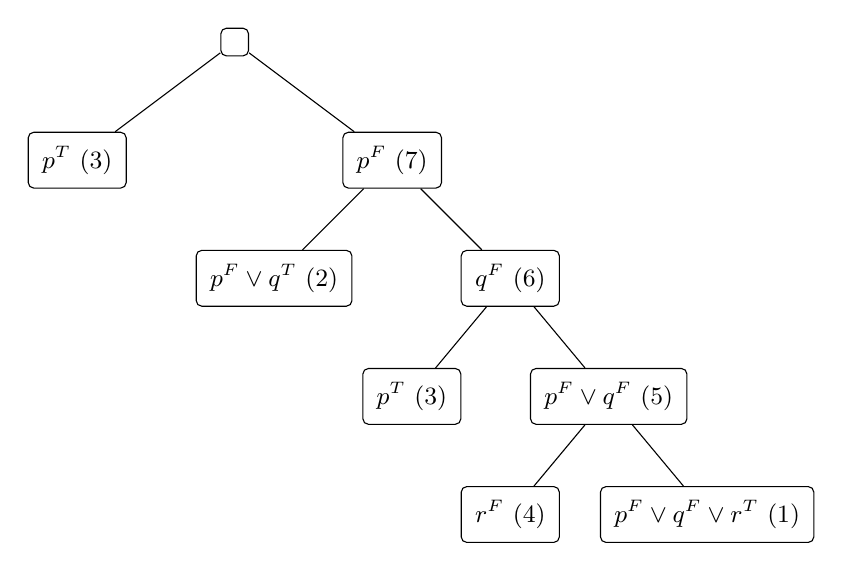
\begin{tikzpicture}[
  level distance=1.5cm,
  level 1/.style={sibling distance=4cm},
  level 2/.style={sibling distance=3cm},
  level 3/.style={sibling distance=2.5cm},
  edge from parent/.style={draw, thin},
  every node/.style={
    draw, 
    rectangle, 
    rounded corners=2pt, 
    inner sep=5pt, 
    font=\small
  }
]  
\node {$\square$}
  child {node {$p^T$ (3)}}
  child {node {$p^F$ (7)}
    child {node {$p^F \lor q^T$ (2)}}
    child {node {$q^F$ (6)}
      child {node {$p^T$ (3)}}
      child {node {$p^F \lor q^F$ (5)}
        child {node {$r^F$ (4)}}
        child {node {$p^F \lor q^F \lor r^T$ (1)}}
      }
    }
  };

\end{tikzpicture}    
\end{tcolorbox}
\caption{Resolution Proof Tree}
\label{fig:r0_proof_tree}
\end{figure}


\begin{figure}[H]
\centering
\begin{tcolorbox}[colback=white, colframe=black, sharp corners, boxrule=0.5pt]
\centering
\begin{tikzpicture}[
    node distance=1.2cm and 0.4cm,
    clause/.style={draw, rectangle, rounded corners=2pt, inner sep=5pt, font=\small, minimum width=1.8cm, fill=white},
    arrow/.style={-{Stealth[scale=1.2]}, thin, color=gray!90}
]

\node[clause] (c3) {3: $p^T$};
\node[clause, right=of c3] (c1) {1: $p^F \lor q^F \lor r^T$};
\node[clause, right=of c1] (c4) {4: $r^F$};
\node[clause, right=of c4] (c2) {2: $p^F \lor q^T$};

\node[clause, below=1.5cm of c1, xshift=1cm] (c5) {5: $p^F \lor q^F$};
\draw[arrow] (c1) -- (c5);
\draw[arrow] (c4) -- (c5);

\node[clause, below=3.5cm of c3, xshift=1.5cm] (c6) {6: $q^F$};
\draw[arrow] (c3) -- (c6);
\draw[arrow] (c5) -- (c6);

\node[clause, below=5.5cm of c2, xshift=-1cm] (c7) {7: $p^F$};
\draw[arrow] (c6) -- (c7);
\draw[arrow] (c2) -- (c7);

\node[clause, below=7.5cm of c3, xshift=3.5cm] (empty) {$\square$};
\draw[arrow] (c7) -- (empty);
\draw[arrow] (c3) .. controls +(down:6cm) and +(left:2cm) .. (empty);

\end{tikzpicture}
\end{tcolorbox}
\caption{Resolution Proof Graph}
\label{fig:r0_proof_graph}
\end{figure}

\definition{Clause Set Simplification}{
Let $\Delta$ be a \linkterm{clause set}{clause_set}, $l \in \Delta$ is a \linkterm{unit clause}{clause_resolution}, and $\Delta'$ be $\Delta$ where 
\begin{itemize}
    \item all \linkterm{clauses}{clause_resolution} $l \lor C$ have been removed, and 
    \item all \linkterm{clauses}{clause_resolution} $\bar{l} \lor C$ have been shortened to $C$.
\end{itemize}
Then $\Delta$ is \linkterm{satisfiable}{satisfiable_ls} iff $\Delta'$ is.

We call $\Delta'$ the \textbf{clause set simplification} of $\Delta$ w.r.t. $l$.
}{clause_set_simplification}

\textbf{Note: }as long as we have \linkterm{unit clauses}{clause_resolution}, we can apply \linkterm{clause set simplification}{clause_set_simplification} recursively, if we can derive the \linkterm{empty clause}{clause_resolution}, we have a \linkterm{proof}{proofs}!

\textbf{Example: }Let $\Delta := \set{p^F \lor q^F \lor r^T , p^F \lor q^T , p^T , r^F}$ 
\begin{itemize}
    \item Choose a \linkterm{unit clause}{clause_resolution}, say $p^T$
    \item Remove any \linkterm{clause}{clause_resolution} with $p^T$ and shorten any \linkterm{clause}{clause_resolution} with $p^F \lor C$ to just $C$
    \item $\Delta' := \set{q^F \lor r^T ,q^T , r^F}$
    \item Choose a \linkterm{unit clause}{clause_resolution}, say $q^T$
    \item Remove any \linkterm{clause}{clause_resolution} with $q^T$ and shorten any \linkterm{clause}{clause_resolution} $q^F \lor C$ to just $C$
    \item $\Delta'' := \set{r^T , r^F}$
    \item Choose any \linkterm{unit clause}{clause_resolution}, say $r^T$
    \item Remove any \linkterm{clause}{clause_resolution} with $r^T$ and shorten any \linkterm{clause}{clause_resolution} $r^F \lor C$ to just $C$
    \item $\Delta''' := \set{\square}$
\end{itemize}
Using \linkterm{clause set simplification}{clause_set_simplification}, we \linkterm{derived}{c_derivation} the \linkterm{empty clause}{clause_resolution} without even \linkterm{resolving}{R0}!

\commandnote{
If we apply \linkterm{clause set simplification}{clause_set_simplification} to a \linkterm{satisfiable}{satisfiable_ls} \linkterm{clause set}{clause_set}, we can read off the \linkterm{model}{model_pl0} that \linkterm{satisfies}{satisfiable_ls} the \linkterm{clause set}{clause_set} (and we will end up with an empty \linkterm{set}{def:set} of clauses, not the the \linkterm{set}{def:set} containing the \linkterm{empty clause}{clause_resolution}). For example, consider $\Delta := \set{p^T ,  q^T \lor r^T , r^F}$
\begin{itemize}
    \item Choose a \linkterm{unit clause}{clause_resolution}, say $p^T$
    \item $\Delta' := \set{q^T \lor r^T , r^F}$
    \item Choose a \linkterm{unit clause}{clause_resolution}, say $r^F$
    \item $\Delta'' := \set{q^T}$
    \item Choose a \linkterm{unit clause}{clause_resolution}, say $q^T$
    \item $\Delta''' := \emptyset$
\end{itemize}
The \linkterm{unit clauses}{clause_resolution} we chose on the way correspond to the \linkterm{model}{model_pl0} $\varphi$ that \linkterm{satisfies}{satisfiable_ls} the \linkterm{clause set}{clause_set}, namely $\varphi := \set{p \mapsto T, r \mapsto F, q \mapsto T}$. Which makes sense since $p \land (q \lor r) \land \neg r$ is indeed \linkterm{satisfiable}{satisfiable_ls} under $\varphi$.
}

\textbf{Example: Resolution in the real world}

Consider we have a knowledge base $\text{KB} := \set{A \Rightarrow B \lor C , A, \neg B}$, we want to check if $\text{KB} \vDash C$. $\text{KB} \vDash C$ iff $\text{KB} \cup \set{\neg C}$ is \linkterm{unsatisfiable}{unsatisfiable_ls}.

First we need to compute $\text{CNF}_0 (A \Rightarrow B \lor C)$
\begin{itemize}
    \item $\text{CNF}_0 (A \Rightarrow B \lor C) = \neg A \lor B \lor C$
\end{itemize}
$\text{KB} \cup \set{\neg C} := \set{\neg A \lor B \lor C, A, \neg B, \neg C} := \set{A^F \lor B^T \lor C^T, A^T, B^F, C^F}$

\begin{figure}[H]
\begin{tcolorbox}[colback=white, colframe=black, sharp corners, boxrule=0.5pt]
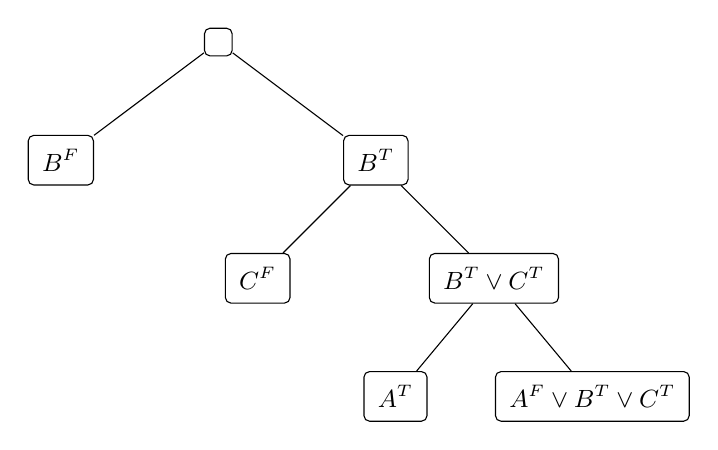
\begin{tikzpicture}[
  level distance=1.5cm,
  level 1/.style={sibling distance=4cm},
  level 2/.style={sibling distance=3cm},
  level 3/.style={sibling distance=2.5cm},
  edge from parent/.style={draw, thin},
  every node/.style={
    draw, 
    rectangle, 
    rounded corners=2pt, 
    inner sep=5pt, 
    font=\small
  }
]  
\node {$\square$}
  child {node {$B^F$}}
  child {node {$B^T$}
    child {node {$C^F$}}
    child {node {$B^T \lor C^T$}
      child {node {$A^T$}}
      child {node {$A^F \lor B^T \lor C^T$}
      }
    }
  };

\end{tikzpicture}  
\hfill
Since $\text{KB} \cup \set{\neg C}$ is \linkterm{unsatisfiable}{unsatisfiable_ls}, $\text{KB} \vDash C$
\end{tcolorbox}
\end{figure}

\definition{SAT}{
Given a \linkterm{propositional formula}{wff0_def} $A$, the \textbf{Boolean Satisfiablity Problem} $\tuple{A, V \subset \mathcal{V}_{\text{PL}^0}}$ is to decide whether or not $A$ is \linkterm{satisfiable}{satisfiable_ls}. We denote the class of all these problems with \textbf{SAT}. \textbf{SAT} problems are NP-Complete. 
}{SAT}

\definition{}{
The tools that address \linkterm{SAT}{SAT} are commonly referred to as \textbf{SAT Solvers}.
}{sat_solver}

\Theorem{
Given any \linkterm{constraint network}{constraint_network} $\gamma := \tuple{V,D,C}$, we can in low-order polynomial time construct a \linkterm{CNF}{cnf} \linkterm{formula}{wff0_def} $A(\gamma)$ that is \linkterm{satisfiable}{satisfiable_ls} iff $\mathcal{\gamma}$ is \linkterm{solvable}{csp_solution}.
}{csp_as_sat}

\minititle{\linkterm{SAT}{SAT} $\to$ \linkterm{CSP}{csp}:}
Given a \linkterm{SAT}{SAT} instance $S = \tuple{A, V}$, we define a \linkterm{CSP}{csp} instance $\gamma := \tuple{V',D,C}$ and \linkterm{bijections}{bijective} $f,\inverse{f}$ mapping \linkterm{satisfying}{satisfiable_ls} assignments of $S$ to \linkterm{solutions}{csp_solution} of $\gamma$ and vice versa:

\begin{itemize}
    \item we define $V' := V$.
    \item we define $D := \bigcup_v D_v$ where $D_v := \set{T,F} \quad \forall v \in V'$
    \item the contraints $C$ consist of a single higher-order constraint which is simply the \linkterm{formula}{wff0_def} $\leadsto C := \set{A}$
    \item The \linkterm{bijections}{bijective} $f,\inverse{f}$ are identity mappings because solutions are identical
\end{itemize}

\minititle{\linkterm{CSP}{csp} $\to$ \linkterm{SAT}{SAT}:}
Given a \linkterm{CSP}{csp} instance $\gamma := \tuple{V,D,C}$, we define a \linkterm{SAT}{SAT} instance $S := \tuple{V', A}$ and \linkterm{bijections}{bijective} $f,\inverse{f}$:

\textbf{Variables: }For each $v \in V$ and each value $a \in D_v$, we introduce a new propositional variable $P_{v,a}$, $V'$ contains all those variables:
\[
V' := \set{P_{v,a} \mid v \in V \land a \in D_v}
\]

\textbf{Formula: } The formula $A$ is defined as the conjunction of three sets of constraints:
\[
A \coloneqq \Phi_{\text{at-least-one}} \land \Phi_{\text{at-most-one}} \land \Phi_{\text{consistent}}
\]
\begin{itemize}
    \item \textbf{At-least-one assignment}: Ensures that each variable $v$ is assigned at least one value from its domain $D_v$:
    \[
    \Phi_{\text{at-least-one}} = \bigwedge_{v \in V} \left( \bigvee_{a \in D_v} P_{v,a} \right)
    \]

    \item \textbf{At-most-one assignment}: Ensures that a variable $v$ cannot be assigned more than one value by forbidding all pairs of distinct values:
    \[
    \Phi_{\text{at-most-one}} = \bigwedge_{v \in V} \bigwedge_{\substack{a,b \in D_v \\ a \neq b}} (\neg P_{v,a} \lor \neg P_{v,b})
    \]

    \item \textbf{Consistency}: Ensures only assignments that satisfy the CSP constraints $C_{vw}$ are allowed by forbidding inconsistent pairs $(a,b)$:
    \[
    \Phi_{\text{consistent}} = \bigwedge_{\{v,w\} \subseteq V} \bigwedge_{(a,b) \notin C_{vw}} (\neg P_{v,a} \lor \neg P_{w,b})
    \]
\end{itemize}

\textbf{Bijections: }
\begin{itemize}
    \item $f$ maps a solution $\alpha$ of the \linkterm{CSP}{csp} to a satisfying assignment $\varphi$ for the \linkterm{SAT}{SAT} instance.
    \[
    f(\alpha) = \varphi, \text{ such that }
    \forall v \in V, \forall a \in D_v:
    \varphi(P_{v,a}) = 
    \begin{cases} 
    T & \text{if } \alpha(v) = a \\ 
    F & \text{otherwise} 
    \end{cases}
    \]
    \item $\inverse{f}$ maps a satisfying assignment $\varphi$ back to a \linkterm{solution}{csp_solution} $\alpha$
    \[
    \inverse{f}(\varphi) = \alpha \text{ such that } \forall v \in V : \alpha(v) = a \Leftrightarrow \varphi(P_{v,a}) = T
    \]
\end{itemize}

\definition{UR}{
\textbf{Unit Resolution (UR)} is a \linkterm{test calculus}{test_calculus} consisting of the following \linkterm{inference rule}{inference_rules_logic}:
\[
\infer[\text{UR}]
{C}
{C \lor P^{\alpha} \qquad P^{\beta} \qquad \alpha \neq \beta}
\]
It is a restricted form of \linkterm{$\mathcal{R}_0$}{R0} where at least one of the two \linkterm{clauses}{clause_resolution} is a \linkterm{unit clause}{clause_resolution}.
}{unit_resolution}

\definition{UP}{
\textbf{Unit Propagation (UP)} is an iterative \linkterm{clause set simplification}{clause_set_simplification} technique triggering a chain reaction of \linkterm{simplifications}{clause_set_simplification} using only \linkterm{UR}{unit_resolution}.
}{unit_propagation}

\definition{Splitting}{
The process of picking a variiable $p$ and branching the search into two cases: one where $p$ is assumed to be $T$, and one where $p$ is assumed to be $F$, resulting in a \linkterm{search tree}{tree_search}.
}{splitting_dpll}

\definition{DPLL}{
The \textbf{Davis Putnam (Logemann-Loverland) Procedure (DPLL)} is a \linkterm{SAT solver}{sat_solver} called on a \linkterm{clause set}{clause_set} $\Delta$ and the empty assignments $\epsilon$. It is the standard algorithm foe deciding the \linkterm{satisfiablity}{satisfiable_ls} of a \linkterm{clause set}{clause_set}:
\begin{enumerate}
    \item Perform \linkterm{Unit Propagation}{unit_propagation} until no more \linkterm{unit clauses}{clause_resolution} exists.
    \item Check if the \linkterm{clause set}{clause_set} is empty (\linkterm{satisfiable}{satisfiable_ls}) or contains an \linkterm{empty clause}{clause_resolution} (\linkterm{unsatisfiable}{unsatisfiable_ls})
    \item If neither, perform \linkterm{splitting}{splitting_dpll} on a variable and repeat.
\end{enumerate}
The pseudocode for DPLL algorithm is shown in \Algref{alg:dpll} and \Algref{alg:simplify}.
}{DPLL}

\begin{algorithm}[H]
\caption{DPLL}
\label{alg:dpll}
\begin{algorithmic}[1]

\Function{DPLL}{$\Delta, \varphi$} \Comment{Returns assignment $\varphi$ or unsatisfiable}
    \State $\Delta' \gets \text{copy of } \Delta$
    \State $\varphi' \gets \varphi$
    
    \While{$\Delta'$ contains a unit clause $C = P^\alpha$} \Comment{Unit Propagation}
        \State $\varphi' \gets \varphi' \cup \{P \mapsto \alpha\}$
        \State $\Delta' \gets \Call{Simplify}{\Delta', P^{\alpha}}$
    \EndWhile

    \If{$\square \in \Delta'$} \Comment{Termination Test: Contradiction}
        \State \Return unsatisfiable
    \EndIf
    
    \If{$\Delta' = \emptyset$} \Comment{Termination Test: Success}
        \State \Return $\varphi'$
    \EndIf

    \State $P \gets \Call{Select-Unassigned-Variable}{\Delta', \varphi'}$ \Comment{Splitting Rule}
    
    \State $\varphi'' \gets \varphi' \cup \{P \mapsto T\}$
    \State $\Delta'' \gets \Call{Simplify}{\Delta', P^T}$
    \State $res \gets \Call{DPLL}{\Delta'', \varphi''}$
    
    \If{$res \neq \text{unsatisfiable}$}
        \State \Return $res$
    \EndIf
    
    \State $\varphi'' \gets \varphi' \cup \{P \mapsto F\}$
    \State $\Delta'' \gets \Call{Simplify}{\Delta', P^F}$
    \State \Return \Call{DPLL}{$\Delta''$, $\varphi''$}
\EndFunction

\end{algorithmic}
\end{algorithm}

\begin{algorithm}[H]
\caption{Simplify}
\label{alg:simplify}
\begin{algorithmic}[1]

\Function{Simplify}{$\Delta, P^\alpha$}
    \State $\Delta' \gets \emptyset$

    \For{each clause $C \in \Delta$}
        \If{$P^\alpha \in C$} 
            \State \textbf{continue} \Comment{Remove any clause that has $P^\alpha$}
        \ElsIf{$P^\beta \in C$}
            \State $C' \gets C \setminus \{P^\beta\}$ \Comment{Remove $P^\beta$ from the clause and keep the rest}
            \State $\Delta' \gets \Delta' \cup \{C'\}$
        \Else
            \State $\Delta' \gets \Delta' \cup \{C\}$ \Comment{Clause does not contain the variable $P$ at all}
        \EndIf
    \EndFor
    \State \Return $\Delta'$
\EndFunction

\end{algorithmic}
\end{algorithm}

\textbf{DPLL Example:} Let $\Delta := \set{p^T \lor q^T \lor r^F , p^F \lor q^F, p^T \lor q^F, r^T}$
\begin{itemize}
\item We start with the empty assignments $\varphi := \emptyset$
\item We see a \linkterm{unit clause}{clause_resolution} $r^T$, we assign $r$ to $T$, hence $\varphi := \set{r \mapsto T}$
\item We apply \linkterm{UP}{unit_propagation} $\leadsto$ $\Delta' := \set{p^T \lor q^T , p^F \lor q^F, p^T \lor q^F}$
\item No \linkterm{unit clauses}{clause_resolution} $\leadsto$ apply \linkterm{splitting}{splitting_dpll}:
\item Choose any variable and branch, say we choose $p$

\begin{minipage}[t]{0.48\linewidth}
    \textbf{Branch 1: Assume $p^T$} \\
    We copy the assignment $\varphi_1 := \set{r \mapsto T}$ and we copy the \linkterm{clause set}{clause_set} $\Delta'_1$
    \begin{itemize}
        \item we treat $p^T$ as a \linkterm{unit clause}{clause_resolution}, hence $\varphi_1 := \set{r \mapsto T, p \mapsto T}$
        \item we apply \linkterm{UP}{unit_propagation} on $\Delta'_1$
        \item $\Delta''_1 := \set{q^F}$
        \item we see a \linkterm{unit clause}{clause_resolution} $q^F$, we assign, $\varphi_1 := \set{r \mapsto T, p \mapsto T, q \mapsto F}$
        \item we apply \linkterm{UP}{unit_propagation} on $\Delta''$
        \item $\Delta'''_1 := \emptyset$
        \item we return \linkterm{satisfiable}{satisfiable_ls} with $\varphi_1$  
    \end{itemize}
\end{minipage}
\hfill
\vrule
\hfill
% --- RIGHT BRANCH: p = F ---
\begin{minipage}[t]{0.48\linewidth}
    \textbf{Branch 2: Assume $p^F$} \\
    We copy the assignment $\varphi_2 := \set{r \mapsto T}$ and we copy the \linkterm{clause set}{clause_set} $\Delta'_2$
    \begin{itemize}
        \item we treat $p^F$ as a \linkterm{unit clause}{clause_resolution}, hence $\varphi_2 := \set{r \mapsto T, p \mapsto F}$
        \item we apply \linkterm{UP}{unit_propagation} on $\Delta'_2$
        \item $\Delta''_2 := \set{q^T, q^F}$
        \item we choose a \linkterm{unit clause}{clause_resolution}, say $q^T$, we assign, $\varphi_2 := \set{r \mapsto T, p \mapsto F, q \mapsto T}$
        \item we apply \linkterm{UP}{unit_propagation} on $\Delta''_2$
        \item $\Delta'''_2 := \set{\square}$
        \item we return \linkterm{unsatisfiable}{unsatisfiable_ls} for this branch.
    \end{itemize}
\end{minipage}
\end{itemize}

The \linkterm{DPLL}{DPLL} procedure can be visualized as a \linkterm{search tree}{tree_search} as shown in \figref{fig:dpll_search_tree}

\begin{figure}[H]
\centering
\begin{tcolorbox}[colback=white, colframe=black, sharp corners, boxrule=0.5pt]
\centering
\begin{tikzpicture}[
    node distance=1.2cm and 1.5cm,
    clause_node/.style={draw, rectangle, rounded corners, inner sep=4pt, font=\footnotesize, align=center, fill=white},
    split_node/.style={draw, diamond, aspect=2, inner sep=2pt, font=\footnotesize, fill=blue!5},
    edge_label/.style={font=\scriptsize, fill=white, inner sep=2pt},
    arrow/.style={-{Stealth[scale=1.0]}, thick}
]

% Level 0: Start
\node[clause_node] (n0) {$\Delta = \{p^T \lor q^T \lor r^F , p^F \lor q^F, p^T \lor q^F, r^T\}$};

% Level 1: Initial UP
\node[clause_node, below=of n0] (n1) {$\Delta' = \{p^T \lor q^T, p^F \lor q^F, p^T \lor q^F\}$};
\draw[arrow] (n0) -- node[edge_label] {UP: $r \mapsto T$} (n1);

% Level 2: The Split on P
\node[split_node, below=of n1] (splitP) {Split $p$};
\draw[arrow] (n1) -- (splitP);

% Level 3: Branches
% Left Branch (p=T)
\node[clause_node, below left=1.5cm and 2.5cm of splitP] (pT_1) {$\Delta'_1 = \{p^T \lor q^T, p^F \lor q^F, p^T \lor q^F\}$};
\node[clause_node, below=of pT_1] (pT_2) {$\Delta''_1 = \{q^F\}$};
\node[clause_node, below=of pT_2] (pT_3) {$\Delta'''_1 = \emptyset$};
\node[draw, rectangle, fill=green!10, below=0.8cm of pT_3] (sat) {\textbf{SAT}};

\draw[arrow] (splitP) -| node[edge_label, pos=0.25] {$p \mapsto T$} (pT_1);
\draw[arrow] (pT_1) -- node[edge_label] {UP: $p \mapsto T$} (pT_2);
\draw[arrow] (pT_2) -- node[edge_label] {UP: $q \mapsto F$} (pT_3);
\draw[arrow] (pT_3) -- (sat);

% Right Branch (p=F)
\node[clause_node, below right=1.5cm and 2.5cm of splitP] (pF_1) {$\Delta'_2 = \{p^T \lor q^T, p^F \lor q^F, p^T \lor q^F\}$};
\node[clause_node, below=of pF_1] (pF_2) {$\Delta''_2 = \{q^T, q^F\}$};
\node[split_node, below=of pF_2] (splitQ) {Split $q$};
\node[clause_node, below=of splitQ] (pF_3) {$\Delta'''_2 = \{\square\}$};
\node[draw, rectangle, fill=red!10, below=0.8cm of pF_3] (unsat) {\textbf{UNSAT}};

\draw[arrow] (splitP) -| node[edge_label, pos=0.25] {$p \mapsto F$} (pF_1);
\draw[arrow] (pF_1) -- node[edge_label] {UP: $p \mapsto F$} (pF_2);
\draw[arrow] (pF_2) -- (splitQ);
\draw[arrow] (splitQ) -- node[edge_label] {$q \mapsto T$} (pF_3);
\draw[arrow] (pF_3) -- (unsat);

\end{tikzpicture}
\end{tcolorbox}
\caption{DPLL Search Tree}
\label{fig:dpll_search_tree}
\end{figure}


\Theorem{
\linkterm{UP}{unit_propagation} is \linkterm{sound}{sound}
}{up_sound}

\Theorem{
\linkterm{UR}{unit_resolution} is \linkterm{refutation}{resolution_refutation}-\linkterm{sound}{sound} (\textit{since \linkterm{$\mathcal{R}_0$}{R0} is})
}{ur_sound}

\Theorem{
\linkterm{UR}{unit_resolution} is not \linkterm{refutation}{resolution_refutation}-\linkterm{complete}{complete}
}{ur_not_complete}
\begin{itemize}
    \item[ ] \textit{Proof Sketch:} \linkterm{UR}{unit_resolution} makes only limited inference, as long as there are \linkterm{unit clauses}{clause_resolution}. It does not guarantee to infer everything that can be inferred
\end{itemize}

\Theorem{
If \linkterm{DPLL}{DPLL} returns \linkterm{unsatisfiable}{unsatisfiable_ls} on $\Delta$, then $\Delta \vdash_{\linkterm{\mathcal{R}_0}{R0}} \square$ with a \linkterm{$\mathcal{R}_0$-refutation}{resolution_refutation}
}{thm_dpll_r0}

\textbf{Observation: }we can read of a \linkterm{resolution proof}{resolution_refutation} from a \linkterm{DPLL}{DPLL} trace. From a (top-down) \linkterm{DPLL}{DPLL} \linkterm{tree}{tree}, we generate a (bottom-up) \linkterm{resolution proof}{resolution_refutation} as shown in \figref{fig:dpll_vs_resolution}. 

\begin{figure}[H]
    \centering
    \begin{tcolorbox}[colback=white, colframe=black, sharp corners, boxrule=0.5pt]
    \begin{minipage}[t]{0.48\linewidth}
        \centering
        \textbf{DPLL Search Tree (Top-Down)} \\ \vspace{0.5cm}
        \begin{tikzpicture}[
            node distance=1.2cm,
            state/.style={draw, rectangle, rounded corners, inner sep=4pt, font=\footnotesize, align=center},
            arrow/.style={-{Stealth[scale=1.0]}, thick}
        ]
            % Root
            \node[state] (n0) {$\Delta = \{ p^T \lor q^T, p^T \lor q^F, p^F \}$};
            
            % Step 1: UP p
            \node[state, below=of n0] (n1) {$\Delta' = \{ q^T, q^F \}$};
            \draw[arrow] (n0) -- node[right, font=\tiny] {UP: $p \mapsto F$} (n1);
            
            % Step 2: UP q
            \node[state, below=of n1] (n2) {$\Delta'' = \{ \square \}$};
            \draw[arrow] (n1) -- node[right, font=\tiny] {UP: $q \mapsto T$} (n2);
            
            % Result
            \node[draw, rectangle, fill=red!10, below=0.6cm of n2] (unsat) {\textbf{UNSAT}};
            \draw[arrow] (n2) -- (unsat);
        \end{tikzpicture}
    \end{minipage}
    \hfill
    \vrule
    \hfill
    % --- RIGHT SIDE: RESOLUTION TREE ---
    \begin{minipage}[t]{0.48\linewidth}
        \centering
        \textbf{Resolution Proof (Bottom-Up)} \\ \vspace{0.5cm}
        \begin{tikzpicture}[
            level 1/.style={sibling distance=5cm}, % Space between q^T and q^F
            level 2/.style={sibling distance=2.5cm}, % Space between the p clauses
            every node/.style={font=\footnotesize},
            edge from parent/.style={draw, latex-}
        ]
            % Root of proof
            \node {$\square$}
                child { node {$q^T$} 
                    child { node {$p^T \lor q^T$} }
                    child { node {$p^F$} }
                }
                child { node {$q^F$} 
                    child { node {$p^T \lor q^F$} }
                    child { node {$p^F$} }
                };
        \end{tikzpicture}
    \end{minipage}
    \end{tcolorbox}
    \caption{DPLL vs Resolution}
    \label{fig:dpll_vs_resolution}
\end{figure}
